% Baccalauréat malgache, série C, 2007 : corrigé.
\TCDBacAttribution{C}{2007}
\providecommand{\cm}{~\mathrm{cm}}
\providecommand{\Plan}{(\mathscr{P})}
\providecommand{\dx}{~\mathrm{d}x}
\providecommand{\dt}{\mathrm{d}t}
\providecommand{\Ouv}{(O;\vec{u},\vec{v})}
\providecommand{\mes}[2]{\mathrm{mes}\left( \widehat{ \overrightarrow{#1} ; \overrightarrow{#2} } \right)}
\providecommand{\D}{(\mathscr{D})}
\providecommand{\Courbe}{(\mathscr{C})}
\providecommand{\Courben}{(\mathscr{C}_n)}
\providecommand{\CourbeU}{(\mathscr{C}_1)}
\providecommand{\CourbeD}{(\mathscr{C}_2)}
\providecommand{\bary}[1]{\mathrm{bar}\left\lbrace #1 \right\rbrace}
\providecommand{\congru}[3]{#1 \equiv #2 \quad \left[ \mathrm{mod}~#3\right]}
\providecommand{\Angl}[2]{\left( \widehat{ \overrightarrow{#1} , \overrightarrow{#2} } \right)}
%
%%%%%%%%%%%%%%%%%%%%%%%%%%%%%%%%%%%%%%%%%%%%%%%%%%%%%%%%%%%%%%%%%%%%%%%%%%%%%%%%%%%%%%%%%%%%%%%%%%%%%%%%%%%%%%%%%%%%%%%%%%%%%%%%
\noindent \underline{\textsc{\textbf{Exercice}}} (4 points)
\begin{description}
	\item[I. ]
	\begin{enumerate}
		\item \vln{Divisibilité de $9^n - 2^n$ par $7$ :}
			Pour $n = 0$ : $9^0 - 2^0 = 0 = 7 \times 0$.
			Supposons $9^n - 2^n = 7k$ avec $k \in \mathbb{Z}$. Alors
			\[
				9^{n+1} - 2^{n+1} = 9 \times 9^n - 2 \times 2^n = 9\left(9^n - 2^n\right) + 7 \times 2^n = 7\left(9k + 2^n\right) .
			\]
			\par\noindent\ansbox{Pour tout $n \in \mathbb{N}$, $7$ divise $9^n - 2^n$.}
		\item \vln{$3n - 2$ et $5n - 3$ sont premiers entre eux :}
			(L'énoncé omet la lettre : il s'agit de tout entier naturel non nul $n$.)
			Pour tout $n$ : $3(5n - 3) - 5(3n - 2) = 15n - 9 - 15n + 10 = 1$.
			Tout diviseur commun de $3n-2$ et $5n-3$ divise donc $1$ ; d'après le théorème de Bézout,
			\par\noindent\ansbox{$\pgcd{3n-2}{5n-3} = 1$ pour tout $n \geq 1$.}
		\item
		\begin{enumerate}
			\item \vln{$\dot{5}$ est solution :}
				$\dot{5}^2 - \dot{5} + \dot{1} = \dot{25} - \dot{5} + \dot{1} = \dot{21} = \dot{0}$ car $21 = 3 \times 7$.
				\par\noindent\ansbox{$\dot{5}$ est solution de (E).}
			\item \vln{Équation équivalente :}
				$(x - \dot{4})^2 = x^2 - \dot{8}x + \dot{16} = x^2 - x + \dot{2}$ car $8 \equiv 1$ et $16 \equiv 2 \pmod 7$.
				Donc $(x - \dot{4})^2 = \dot{1} \iff x^2 - x + \dot{2} = \dot{1} \iff x^2 - x + \dot{1} = \dot{0}$.
				\par\noindent\ansbox{(E) $\iff (x - \dot{4})^2 = \dot{1}$.}
			\item \vln{Ensemble $S$ :}
				Dans $\mathbb{Z}/7\mathbb{Z}$, les carrés sont $\dot{0}^2 = \dot{0}$, $(\pm\dot{1})^2 = \dot{1}$, $(\pm\dot{2})^2 = \dot{4}$, $(\pm\dot{3})^2 = \dot{2}$ :
				$y^2 = \dot{1} \iff y = \dot{1}$ ou $y = -\dot{1} = \dot{6}$.
				Donc $x - \dot{4} = \dot{1}$ ou $x - \dot{4} = \dot{6}$, soit $x = \dot{5}$ ou $x = \dot{3}$ (on vérifie : $9 - 3 + 1 = 7$).
				Les entiers $x$ cherchés sont ceux qui sont congrus à $3$ ou à $5$ modulo $7$ et vérifient $-7 < x < 7$ :
				$x \in \{3 ; 3 - 7\} = \{3 ; -4\}$ ou $x \in \{5 ; 5 - 7\} = \{5 ; -2\}$.
				\par\noindent\ansbox{$S = \{-4 \, ; -2 \, ; 3 \, ; 5\}$.}
		\end{enumerate}
	\end{enumerate}
	\item[II. ]
	L'urne contient $20$ boules : $10$ blanches, $6$ noires, $4$ vertes.
	Les nombres premiers entre $1$ et $20$ sont $2, 3, 5, 7, 11, 13, 17, 19$ (huit numéros) ;
	les multiples de $7$ sont $7$ et $14$.
	\begin{enumerate}
		\item Tirage successif sans remise : $20 \times 19 = 380$ résultats équiprobables (arrangements).
		\begin{itemize}
			\item \vln{Événement $A$ :}
				deux blanches : $10 \times 9 = 90$ ; deux noires : $6 \times 5 = 30$ ; deux vertes : $4 \times 3 = 12$.
				$P(A) = \frac{132}{380}$, soit \par\noindent\ansbox{$P(A) = \frac{33}{95}$.}
			\item \vln{Événement $B$ :}
				deux numéros premiers distincts : $8 \times 7 = 56$ résultats.
				$P(B) = \frac{56}{380}$, soit \par\noindent\ansbox{$P(B) = \frac{14}{95}$.}
		\end{itemize}
		\item Tirage successif avec remise : $20^2 = 400$ résultats équiprobables.
		\begin{itemize}
			\item \vln{Événement $C$ :}
				L'événement contraire est « aucune boule blanche » : $10 \times 10 = 100$ résultats.
				$P(C) = 1 - \frac{100}{400}$, soit \par\noindent\ansbox{$P(C) = \frac{3}{4}$.}
			\item \vln{Événement $D$ :}
				Les deux numéros sont dans $\{7 ; 14\}$ : $2 \times 2 = 4$ résultats.
				$P(D) = \frac{4}{400}$, soit \par\noindent\ansbox{$P(D) = \frac{1}{100}$.}
		\end{itemize}
	\end{enumerate}
\end{description}
%%%%%%%%%%%%%%%%%%%%%%%%%%%%%%%%%%%%%%%%%%%%%%%%%%%%%%%%%%%%%%%%%%%%%%%%%%%%%%%%%%%%%%%%%%%%%%%%%%%%%%%%%%%%%%%%%%%%%%%%%%%%%%%%
\noindent \underline{\textsc{\textbf{PROBLEME I}}} (7 points)
\begin{description}
	\item[Partie A]
	\begin{enumerate}
		\item \vln{Figure :}
			Les carrés $ABCD$ et $DEFG$ sont directs ; $E$ est le milieu de $[CD]$, donc $DE = 3\cm$ et $G$ est l'image de $E$ par la rotation de centre $D$ et d'angle $\frac{\pi}{2}$.
			\begin{center}
			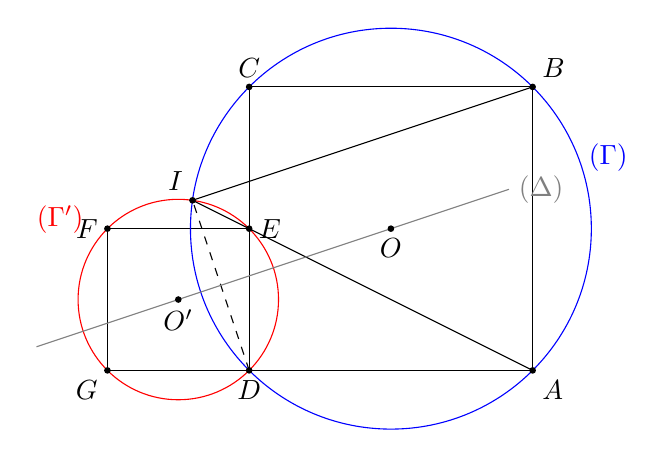
\begin{tikzpicture}[scale=.6,>=stealth]
				\coordinate (A) at (6,0); \coordinate (B) at (6,6); \coordinate (C) at (0,6); \coordinate (D) at (0,0);
				\coordinate (E) at (0,3); \coordinate (F) at (-3,3); \coordinate (G) at (-3,0);
				\coordinate (O) at (3,3); \coordinate (O') at (-1.5,1.5); \coordinate (I) at (-1.2,3.6);
				\draw (A) -- (B) -- (C) -- (D) -- cycle;
				\draw (D) -- (E) -- (F) -- (G) -- cycle;
				\draw[blue] (O) circle (4.2426);
				\draw[red] (O') circle (2.1213);
				\draw[thin] (A) -- (I); \draw[thin] (B) -- (I);
				\draw[dashed] (D) -- (I);
				\draw[gray] (-4.5,0.5) -- (5.5,3.833) node[right] {$(\Delta)$};
				\foreach \P/\L/\pos in {A/A/below right,B/B/above right,C/C/above,D/D/below,E/E/right,F/F/left,G/G/below left,O/O/below,O'/O'/below,I/I/above left}
					\fill (\P) circle (2pt) node[\pos] {$\L$};
				\node[blue] at (7.6,4.5) {$(\Gamma)$};
				\node[red] at (-4,3.2) {$(\Gamma')$};
			\end{tikzpicture}
			\end{center}
		\item
		\begin{enumerate}
			\item \vln{Rapport et angle de $S$ :}
				$S(D) = D$ et $S(A) = B$ : le rapport est $\frac{DB}{DA} = \frac{6\sqrt{2}}{6} = \sqrt{2}$ (diagonale du carré) et l'angle est
				$\Angl{DA}{DB} = \frac{\pi}{4}$ (la diagonale $[DB]$ est la bissectrice de l'angle droit direct $\widehat{ADC}$).
				\par\noindent\ansbox{$S$ : centre $D$, rapport $\sqrt{2}$, angle $\frac{\pi}{4}$.}
			\item \vln{Image de $E$ et angle $\Angl{AE}{BF}$ :}
				$DF$ est la diagonale du carré $DEFG$ : $DF = \sqrt{2}\, DE$ et $\Angl{DE}{DF} = \frac{\pi}{4}$ (carré direct).
				Donc \par\noindent\ansbox{$S(E) = F$.}
				Comme $S(A) = B$ et $S(E) = F$, la similitude $S$ transforme le vecteur $\overrightarrow{AE}$ en $\overrightarrow{BF}$ et
				l'angle de ces deux vecteurs est l'angle de $S$ :
				\par\noindent\ansbox{$\mes{AE}{BF} = \frac{\pi}{4} \pmod{2\pi}$.}
		\end{enumerate}
		\item
		\begin{enumerate}
			\item Le point $I$ est placé sur la figure ; les droites $(AE)$ et $(BF)$ se coupent car leur angle n'est pas nul modulo $\pi$.
			\item \vln{$I$ est sur $(\Gamma)$ et sur $(\Gamma')$ :}
				Comme $I \in (AE)$ et $I \in (BF)$ (et $I \neq A$, $I \neq B$), on a, modulo $\pi$ :
				$\mes{IA}{IB} = \mes{AE}{BF} = \frac{\pi}{4} \ [\pi]$.
				Or $\mes{CA}{CB} = \frac{\pi}{4}$ (la diagonale $[CA]$ fait un angle de $\frac{\pi}{4}$ avec le côté $[CB]$, dans le sens direct). D'après le rappel,
				$A$, $B$, $C$, $I$ sont cocycliques : $I \in (\Gamma)$.

				De même, $\mes{IE}{IF} = \mes{AE}{BF} = \frac{\pi}{4} \ [\pi]$ et $\mes{DE}{DF} = \frac{\pi}{4}$, donc $D$, $E$, $F$, $I$ sont cocycliques : $I \in (\Gamma')$.

				Les cercles $(\Gamma)$ et $(\Gamma')$ sont distincts et ont en commun $D$ et $I$ ; $I \neq D$ car $D \notin (AE)$.
				\par\noindent\ansbox{$I$ est le second point d'intersection de $(\Gamma)$ et $(\Gamma')$ (l'autre étant $D$).}
			\item \vln{$(ID) \perp (BF)$ :}
				$[DF]$ est une diagonale du carré $DEFG$, donc un diamètre de $(\Gamma')$. Le point $I$ de $(\Gamma')$, distinct de $D$ et de $F$,
				voit ce diamètre sous un angle droit : $(ID) \perp (IF)$. Comme $(IF) = (BF)$,
				\par\noindent\ansbox{les droites $(ID)$ et $(BF)$ sont perpendiculaires.}
		\end{enumerate}
		\item \vln{$S_\Delta(D) = I$ :}
			$D$ et $I$ sont sur $(\Gamma)$ de centre $O$ : $OD = OI$ ; ils sont sur $(\Gamma')$ de centre $O'$ : $O'D = O'I$.
			Donc $O$ et $O'$ (distincts) sont sur la médiatrice de $[DI]$, qui est donc la droite $(OO') = (\Delta)$.
			\par\noindent\ansbox{$I$ est le symétrique de $D$ par rapport à $(\Delta)$ : $S_\Delta(D) = I$.}
	\end{enumerate}
	\item[Partie B]
	\begin{enumerate}
		\item \vln{Affixes :}
			$\overrightarrow{DA} = 6\vec{e_1}$, $\overrightarrow{DC} = 6\vec{e_2}$, $\overrightarrow{DB} = \overrightarrow{DA} + \overrightarrow{DC}$ ;
			$\overrightarrow{DE} = 3\vec{e_2}$ et $\overrightarrow{DG}$ s'obtient en tournant $\overrightarrow{DE}$ de $\frac{\pi}{2}$ : $z_G = i \times 3i = -3$.
			\par\noindent\ansbox{$z_A = 6$, $z_B = 6 + 6i$, $z_C = 6i$, $z_D = 0$, $z_G = -3$.}
			(Aussi $z_E = 3i$, $z_F = -3 + 3i$, $z_O = 3 + 3i$, $z_{O'} = -\frac{3}{2} + \frac{3}{2} i$.)
		\item
		\begin{enumerate}
			\item \vln{Expression complexe de $S$ :}
				$S : z' = az$ (centre $D$ d'affixe $0$) et $S(A) = B$ : $6a = 6 + 6i$, d'où \par\noindent\ansbox{$S : z' = (1 + i) z$.}
			\item \vln{Éléments caractéristiques :}
				$1 + i = \sqrt{2}\, \expo{i\frac{\pi}{4}}$ : \par\noindent\ansbox{$S$ a pour centre $D$, pour rapport $\sqrt{2}$ et pour angle $\frac{\pi}{4}$.}
				On vérifie $S(E) = (1+i)\,3i = -3 + 3i = z_F$.
		\end{enumerate}
		\item Notons $a = \frac{4}{5} + \frac{3}{5} i$ et $b = -\frac{6}{5} + \frac{18}{5} i$.
		\begin{enumerate}
			\item \vln{Nature de $f$ :}
				$|a| = \sqrt{\frac{16}{25} + \frac{9}{25}} = 1$ : $f$ est un antidéplacement. De plus
				$a\bar{b} = \frac{(4 + 3i)(-6 - 18i)}{25} = \frac{-24 - 72i - 18i + 54}{25} = \frac{6 - 18i}{5} = -b$,
				donc $a\bar{b} + b = 0$ : pour tout $z$, $f(f(z)) = a\overline{a\bar{z} + b} + b = a\bar{a} z + a\bar{b} + b = z$.
				Un antidéplacement involutif est une symétrie orthogonale. Son axe est l'ensemble des points invariants ;
				$f(O) = a(3 - 3i) + b = \frac{21 - 3i}{5} + \frac{-6 + 18i}{5} = 3 + 3i = z_O$ et
				$f(O') = a\left(-\frac{3}{2} - \frac{3}{2}i\right) + b = \frac{-3 - 21i}{10} + \frac{-12 + 36i}{10} = -\frac{3}{2} + \frac{3}{2}i = z_{O'}$.
				\par\noindent\ansbox{$f$ est la symétrie orthogonale d'axe $(\Delta) = (OO')$, c'est-à-dire $f = S_\Delta$.}
			\item \vln{Expression analytique :}
				$z' = \frac{(4 + 3i)(x - iy)}{5} - \frac{6}{5} + \frac{18}{5} i = \frac{4x + 3y - 6}{5} + i\, \frac{3x - 4y + 18}{5}$.
				\par\noindent\ansbox{$x' = \frac{4}{5}x + \frac{3}{5}y - \frac{6}{5}$ et $y' = \frac{3}{5}x - \frac{4}{5}y + \frac{18}{5}$.}
				(L'axe a pour équation $x' = x$, soit $x - 3y + 6 = 0$ : il passe bien par $O(3;3)$ et $O'\left(-\frac{3}{2};\frac{3}{2}\right)$.)
			\item \vln{Affixe de $I$ :}
				$z_I = f(0) = b$ : \par\noindent\ansbox{$z_I = -\frac{6}{5} + \frac{18}{5}\, i$.}
				D'après la partie A, ce point est bien l'intersection de $(AE)$ et $(BF)$ :
				$z_I = 6 + \frac{6}{5}(-6 + 3i)$ et $z_I = 6 + 6i + \frac{4}{5}(-9 - 3i)$.
			\item \vln{Alignement de $G$, $I$, $C$ :}
				$z_I - z_G = \frac{9}{5} + \frac{18}{5} i = \frac{9}{5}(1 + 2i)$ et $z_C - z_G = 3 + 6i = 3(1 + 2i)$.
				Donc $\overrightarrow{GI} = \frac{3}{5}\, \overrightarrow{GC}$ et \par\noindent\ansbox{$G$, $I$, $C$ sont alignés.}
		\end{enumerate}
	\end{enumerate}
\end{description}
%%%%%%%%%%%%%%%%%%%%%%%%%%%%%%%%%%%%%%%%%%%%%%%%%%%%%%%%%%%%%%%%%%%%%%%%%%%%%%%%%%%%%%%%%%%%%%%%%%%%%%%%%%%%%%%%%%%%%%%%%%%%%%%%
\noindent \underline{\textsc{\textbf{PROBLEME II}}} (9 points)
\begin{description}
	\item[Partie A :]
	\begin{description}
		\item[I. ]
		\begin{enumerate}
			\item \vln{Variations et signe de $g$ :}
				$g$ est dérivable sur $[0;+\infty[$ et
				\[
					g'(x) = \frac{1}{x+1} - 1 + x - x^2 = \frac{1 - (x+1) + x(x+1) - x^2(x+1)}{x+1} = \frac{-x^3}{x+1} .
				\]
				Pour $x \geq 0$, $g'(x) \leq 0$ (nul seulement en $0$) : $g$ est strictement décroissante sur $[0;+\infty[$. Comme $g(0) = 0$ :
				\par\noindent\ansbox{$g(x) \leq 0$ pour tout $x \geq 0$.}
			\item \vln{Encadrement :}
				Posons $\varphi(x) = \ln(1+x) - x + \frac{x^2}{2}$ : $\varphi'(x) = \frac{1}{1+x} - 1 + x = \frac{x^2}{1+x} \geq 0$,
				donc $\varphi$ est croissante sur $[0;+\infty[$ et $\varphi(x) \geq \varphi(0) = 0$ :
				\par\noindent\ansbox{$\ln(1+x) - x + \frac{x^2}{2} \geq 0$ pour $x \geq 0$.}
				Ainsi $\ln(1+x) - x \geq -\frac{x^2}{2}$, et, d'après 1., $\ln(1+x) - x \leq -\frac{x^2}{2} + \frac{x^3}{3}$.
				Pour $x > 0$ (le quotient n'est pas défini en $0$), on divise par $x^2 > 0$ :
				\par\noindent\ansbox{$-\frac{1}{2} \leq \frac{\ln(1+x) - x}{x^2} \leq -\frac{1}{2} + \frac{x}{3}$ pour tout $x > 0$.}
		\end{enumerate}
		\item[II. ]
		\begin{enumerate}
			\item
			\begin{enumerate}
				\item \vln{Continuité et dérivabilité en $0$ :}
					$\lim_{x\to 0^+} \frac{\ln(1+x)}{x} = 1 = f(0)$ (limite usuelle) : $f$ est continue à droite en $0$.
					Pour $x > 0$, $\frac{f(x) - f(0)}{x} = \frac{\ln(1+x) - x}{x^2}$, encadré par $-\frac{1}{2}$ et $-\frac{1}{2} + \frac{x}{3}$ ;
					par le théorème des gendarmes, ce taux tend vers $-\frac{1}{2}$.
					\par\noindent\ansbox{$f$ est continue et dérivable à droite en $0$, avec $f'(0) = -\frac{1}{2}$.}
				\item \vln{Tangente $(T)$ :}
					$y = f'(0)(x - 0) + f(0)$ : \par\noindent\ansbox{$(T) : y = -\frac{1}{2}x + 1$.}
				\item \vln{Variations et signe de $h$ :}
					$h'(x) = 1 - \ln(x+1) - (x+1)\frac{1}{x+1} = -\ln(x+1) \leq 0$ sur $[0;+\infty[$ (nul seulement en $0$) :
					$h$ est strictement décroissante, et $h(0) = 0$.
					\par\noindent\ansbox{$h(x) < 0$ pour tout $x > 0$, et $h(0) = 0$.}
				\item \vln{Dérivée de $f$ :}
					Pour $x > 0$ :
					$f'(x) = \frac{\frac{x}{1+x} - \ln(1+x)}{x^2} = \frac{x - (1+x)\ln(1+x)}{x^2(1+x)}$, c'est-à-dire
					\par\noindent\ansbox{$f'(x) = \frac{h(x)}{x^2(1+x)} < 0$ pour $x > 0$, et $f'(0) = -\frac{1}{2}$.}
					$f$ est strictement décroissante sur $[0;+\infty[$.
				\item \vln{Tableau de variation et courbe :}
					$\lim_{x\to+\infty} \frac{\ln(1+x)}{x} = \lim \frac{\ln(1+x)}{1+x} \cdot \frac{1+x}{x} = 0 \times 1 = 0$ : l'axe des abscisses est asymptote.
					\[
					\begin{array}{c|ccc}
						x & 0 & & +\infty \\ \hline
						f'(x) & -\frac{1}{2} & - & \\ \hline
						 & 1 & & \\
						f & & \searrow & \\
						 & & & 0
					\end{array}
					\]
					Quelques valeurs : $f(1) = \ln 2 \approx 0{,}69$ ; $f(2) \approx 0{,}55$ ; $f(4) \approx 0{,}40$.
					D'après I.2., $f(x) \geq 1 - \frac{x}{2}$ : la courbe est au-dessus de $(T)$.
					\begin{center}
					\begin{tikzpicture}[x=2cm,y=2cm,>=stealth]
						\draw[->] (-0.3,0) -- (5.7,0) node[below] {$x$};
						\draw[->] (0,-0.3) -- (0,1.5) node[left] {$y$};
						\foreach \t in {1,2,3,4,5} \draw (\t,0.03) -- (\t,-0.03) node[below] {\small $\t$};
						\draw (0.03,1) -- (-0.03,1) node[left] {\small $1$};
						\node[below left] at (0,0) {$O$};
						\draw[blue,thick] plot[domain=0.001:5.5,samples=100] (\x,{ln(1+\x)/\x});
						\draw[red] (-0.2,1.1) -- (2.4,-0.2) node[right] {$(T)$};
						\node[blue] at (3.5,0.6) {$\Courbe$};
					\end{tikzpicture}
					\end{center}
			\end{enumerate}
			\item \vln{Encadrement de $F(1)$ :}
				Pour $t > 0$, $f(t) = 1 + t\cdot\frac{\ln(1+t) - t}{t^2}$ ; d'après I.2. (multiplié par $t > 0$) :
				$1 - \frac{t}{2} \leq f(t) \leq 1 - \frac{t}{2} + \frac{t^2}{3}$, encore vrai pour $t = 0$.
				En intégrant sur $[0;1]$ :
				\[
					\int_0^1 \left(1 - \frac{t}{2}\right)\dt = 1 - \frac{1}{4} = \frac{3}{4}
					\quad\text{et}\quad
					\int_0^1 \left(1 - \frac{t}{2} + \frac{t^2}{3}\right)\dt = \frac{3}{4} + \frac{1}{9} = \frac{31}{36} .
				\]
				\par\noindent\ansbox{$\frac{3}{4} \leq F(1) \leq \frac{31}{36}$.}
				Conclusion : on obtient une valeur approchée de $F(1)$ (qu'on ne sait pas calculer par primitive) :
				$0{,}75 \leq F(1) \leq 0{,}87$ environ ; par exemple $F(1) \approx \frac{29}{36} \approx 0{,}81$ à $\frac{1}{18} \approx 0{,}06$ près.
				$F(1)$ est aussi l'aire, en unités d'aire, du domaine sous $\Courbe$ entre $x = 0$ et $x = 1$.
		\end{enumerate}
	\end{description}
	\item[Partie B :]
	\begin{description}
		\item[I. ]
		\begin{enumerate}
			\item \vln{$f(I) \subset I$ :}
				$f$ est continue et strictement décroissante sur $[0;1]$, donc $f([0;1]) = [f(1) ; f(0)] = [\ln 2 ; 1]$.
				Comme $0 < \ln 2 < 1$, \par\noindent\ansbox{$f(I) = [\ln 2 ; 1] \subset I$.}
			\item \vln{Équation $f(x) = x$ :}
				Soit $\psi(x) = f(x) - x$ sur $I$ : $\psi$ est continue et strictement décroissante (somme de deux fonctions strictement décroissantes),
				$\psi(0) = 1 > 0$ et $\psi(1) = \ln 2 - 1 < 0$. D'après le théorème des valeurs intermédiaires (bijection),
				\par\noindent\ansbox{l'équation $f(x) = x$ a une unique solution $\alpha \in [0;1]$.}
				(Numériquement $\alpha \approx 0{,}747$ ; $\alpha$ vérifie $\ln(1+\alpha) = \alpha^2$.)
			\item \vln{Étude de $k$ :}
				$k'(x) = 3x^2 + 2x + 2 - 2\ln(x+1) - 2(x+1)\frac{1}{x+1}$, soit \par\noindent\ansbox{$k'(x) = 3x^2 + 2x - 2\ln(x+1)$.}
				$k''(x) = 6x + 2 - \frac{2}{x+1} = \frac{6x^2 + 8x}{x+1} \geq 0$ sur $[0;+\infty[$ : \par\noindent\ansbox{$k'$ est croissante sur $[0;+\infty[$.}
				Comme $k'(0) = 0$, $k'(x) \geq 0$ ; donc $k$ est croissante et, comme $k(0) = 0$,
				\par\noindent\ansbox{$k'(x) \geq 0$ et $k(x) \geq 0$ pour tout $x \geq 0$.}
			\item \vln{$f'(x) + \frac{1}{2} \geq 0$ et $|f'(x)| \leq \frac{1}{2}$ sur $I$ :}
				Pour $x > 0$ :
				\[
					f'(x) + \frac{1}{2} = \frac{2x - 2(1+x)\ln(1+x) + x^2(1+x)}{2x^2(1+x)} = \frac{k(x)}{2x^2(1+x)} \geq 0 ,
				\]
				et pour $x = 0$, $f'(0) + \frac{1}{2} = 0$. \par\noindent\ansbox{$f'(x) + \frac{1}{2} \geq 0$ pour tout $x \geq 0$.}
				Avec II.1.(d), $-\frac{1}{2} \leq f'(x) \leq 0$ sur $[0;+\infty[$, en particulier sur $I$ :
				\par\noindent\ansbox{$|f'(x)| \leq \frac{1}{2}$ pour tout $x \in I$.}
		\end{enumerate}
		\item[II. ]
		\begin{enumerate}
			\item \vln{$U_n \in I$ :}
				$U_0 = 0 \in I$ ; si $U_n \in I$, alors $U_{n+1} = f(U_n) \in f(I) \subset I$.
				\par\noindent\ansbox{Pour tout $n$, $U_n \in I$.}
			\item \vln{Inégalité des accroissements finis :}
				$f$ est dérivable sur $I$ avec $|f'| \leq \frac{1}{2}$ ; $U_n$ et $\alpha$ sont dans $I$, donc
				$|f(U_n) - f(\alpha)| \leq \frac{1}{2}|U_n - \alpha|$. Comme $f(U_n) = U_{n+1}$ et $f(\alpha) = \alpha$ :
				\par\noindent\ansbox{$|U_{n+1} - \alpha| \leq \frac{1}{2}|U_n - \alpha|$.}
			\item \vln{Majoration :}
				Par récurrence : $|U_0 - \alpha| = \alpha \leq 1 = \frac{1}{2^0}$ ; si $|U_n - \alpha| \leq \frac{1}{2^n}$, alors
				$|U_{n+1} - \alpha| \leq \frac{1}{2} \cdot \frac{1}{2^n} = \frac{1}{2^{n+1}}$.
				\par\noindent\ansbox{$|U_n - \alpha| \leq \frac{1}{2^n}$ pour tout $n \in \mathbb{N}$.}
			\item \vln{Limite :}
				$\lim_{n\to+\infty} \frac{1}{2^n} = 0$ (car $0 < \frac{1}{2} < 1$), donc $|U_n - \alpha| \to 0$.
				\par\noindent\ansbox{$\lim_{n\to+\infty} U_n = \alpha$.}
		\end{enumerate}
	\end{description}
\end{description}
